\section{React}

\textit{React} (oder \textit{React.js}) ist eine Front-End JavaScript-Library zum Erstellen von Nutzerinterfaces, welche von Facebook entwickelt wird. Neben \textit{Vue.js} und \textit{Angular} ist React eine der bekanntesten und am weitesten verbreiteten Front-End-Lösungen für moderne Web-Anwendungen. \cite{nadafkhanrathod2020}

Sokka nutzt React als Lösung für das \nameref{acp}.

\subsection{JSX}

Ein Vorteil von React gegenüber anderen bekannten Front-End-Libraries ist \textbf{JSX}, in der Langform \textit{JavaScript-XML}. JSX erlaubt es, HTML in JavaScript-Code zu verwenden und vice versa. Beispielsweise kann eine Information von einer API geladen und anschließend mit Hilfe von JSX in HTML angezeigt werden.

\begin{code}[h]
    \centering
    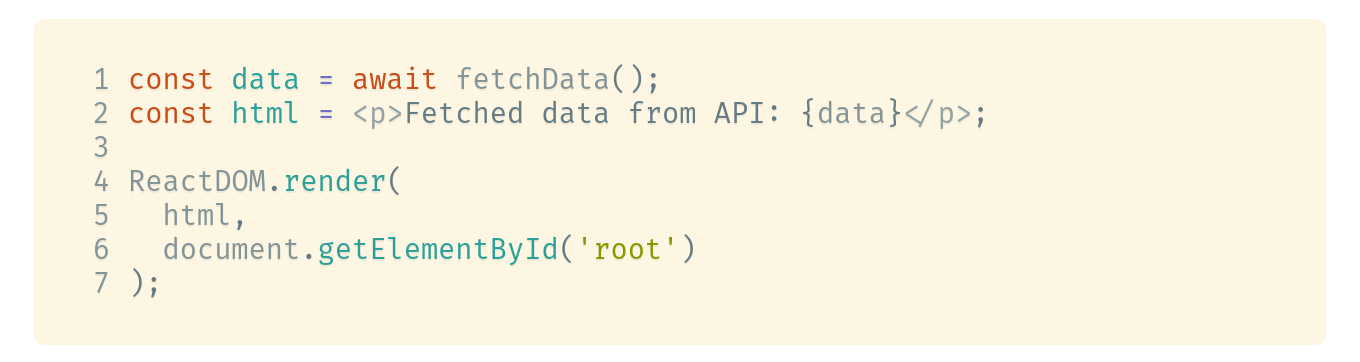
\includegraphics[width=1\textwidth]{images/React/jsx.png}
    \vspace{-25pt}
    \caption{JSX-Beispiel für das Laden und Rendern von Informationen}
\end{code}

\subsection{Components}

In React ist alles ein \textbf{Component}. Jede Reihe, jede Spalte, jeder Kasten, jedes Eingabefeld und jeder Knopf sind ein eigenes Component.

\begin{figure}[h]
    \begin{center}
        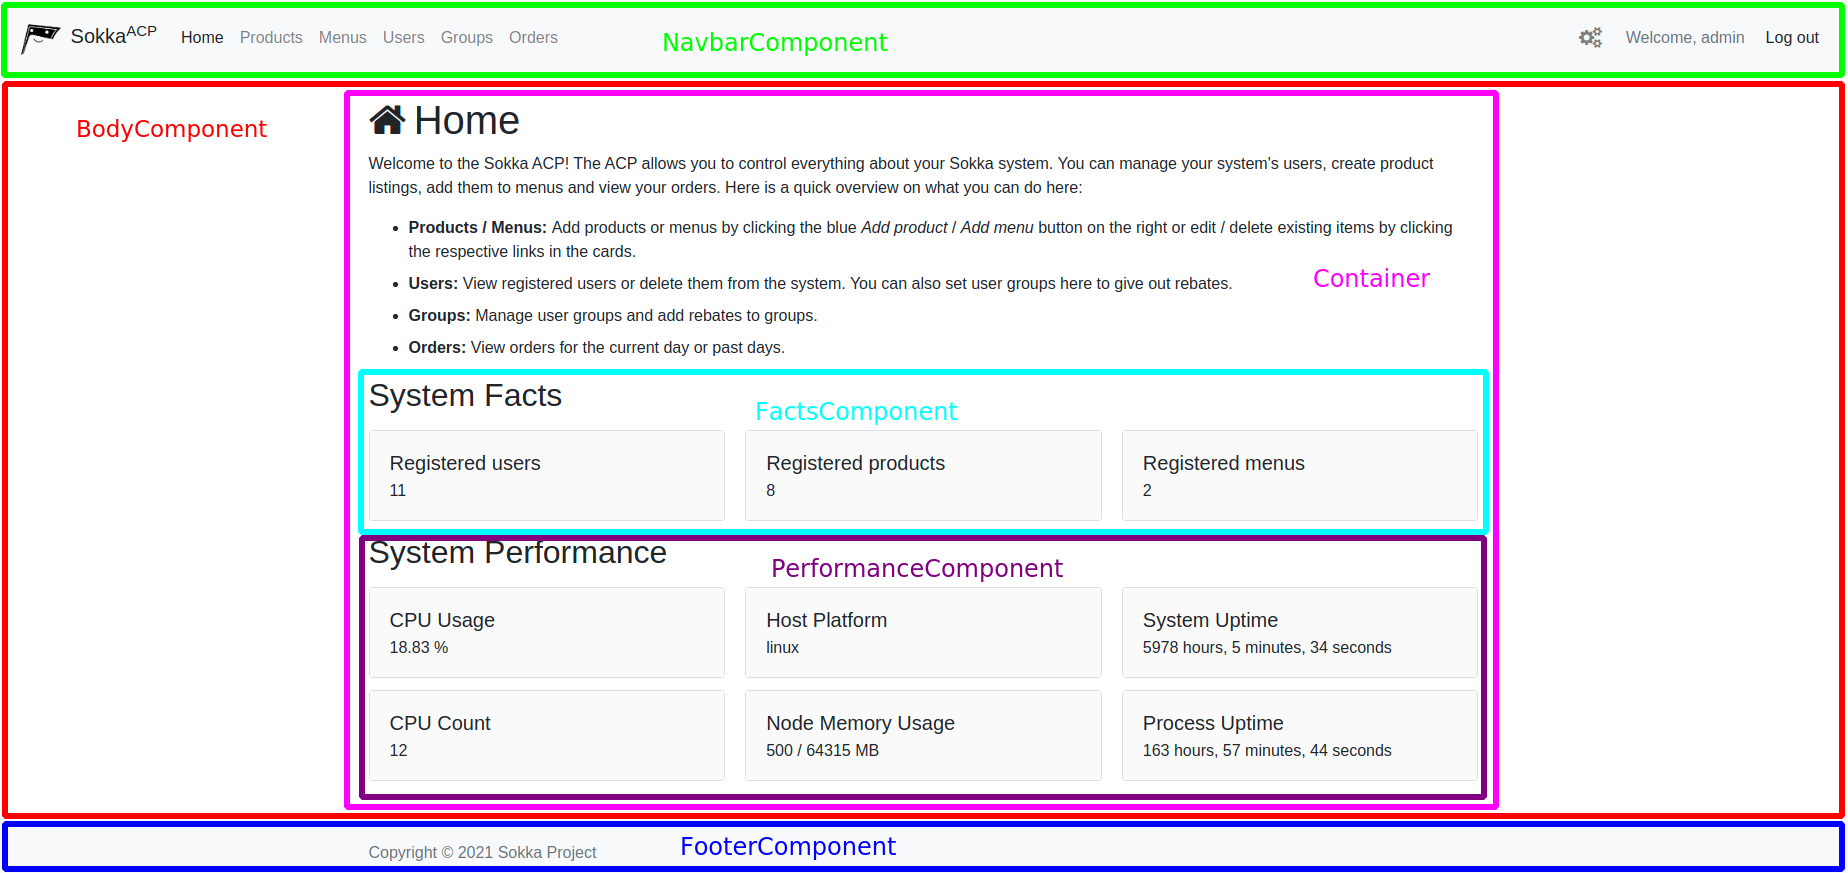
\includegraphics[width=0.75\textwidth]{images/React/components.png}
        \caption{JSX-Components am Beispiel des Sokka-ACPs}
    \end{center}
\end{figure}

Components können ineinander und so oft wie man möchte verwendet werden, womit man sich eine Menge Code spart. Wenn man das Verhalten eines Components dennoch der Situation entsprechend ändern möchte, können \textbf{Component Properties} übergeben werden. Diese Properties oder auch \lstinline{props} versorgen eine neu erstellte Komponente also mit initialen Informationen, welche für das Rendern der Component notwendig sind.

\begin{code}[h]
    \centering
    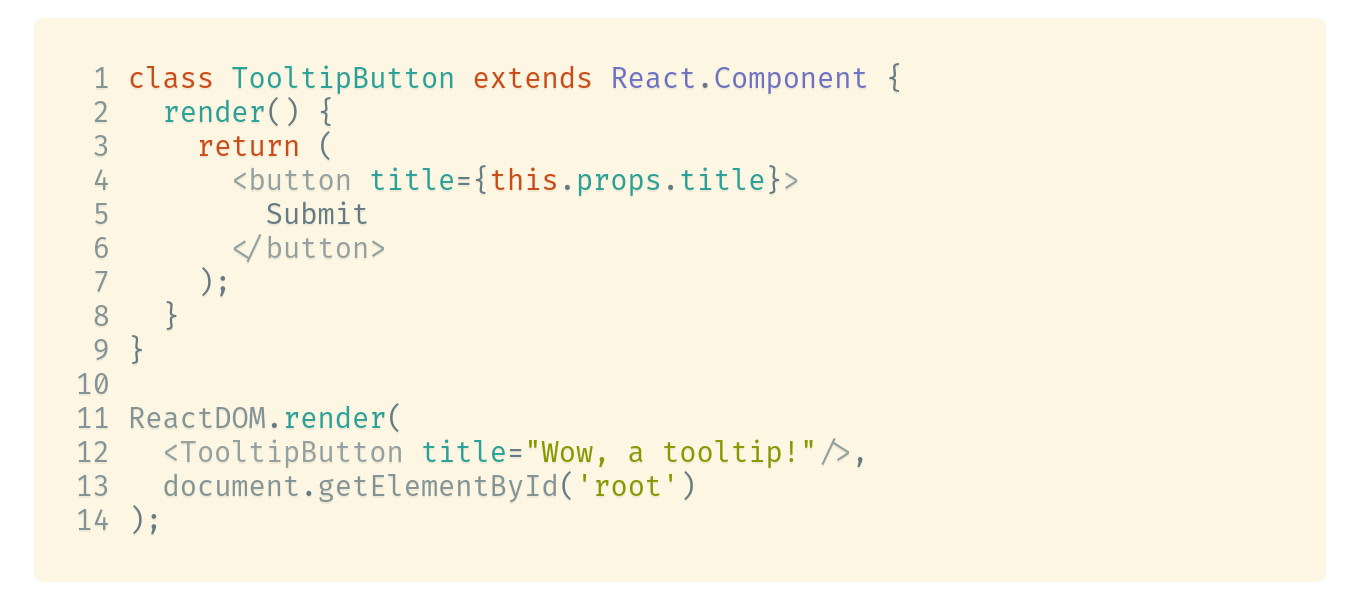
\includegraphics[width=1\textwidth]{images/React/button.png}
    \vspace{-25pt}
    \caption{Beispiel für ein React-Component für einen Button mit änderbarem Tooltip}
\end{code}

\subsection{States}

Oftmals reicht es nicht aus, eine Component nur mit initialen Informationen zu versorgen. Manche Components halten bestimmte Daten, welche sich über die Zeit ändern, weil sie zum Beispiel nachgeladen oder durch den Nutzer geändert werden. Für solche Daten gibt es in Components die \textbf{Component States}.

\begin{code}[h]
    \centering
    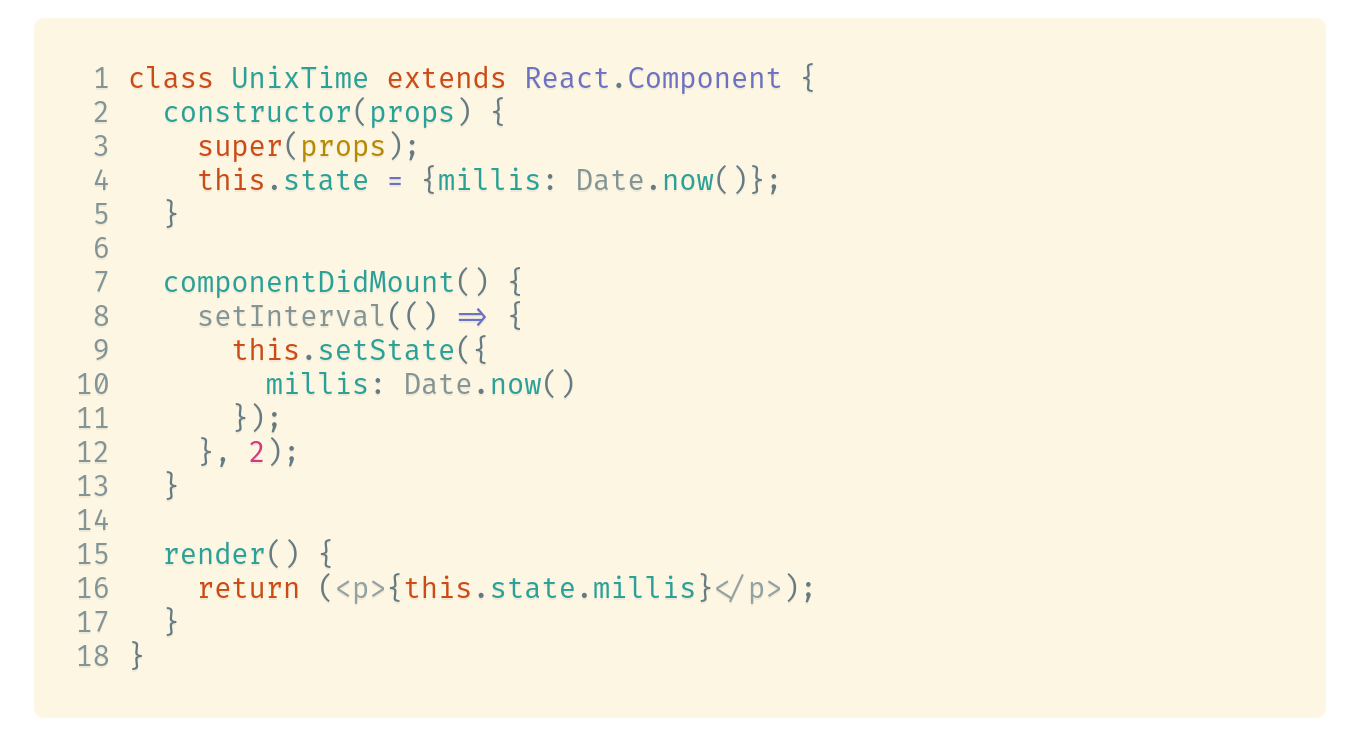
\includegraphics[width=0.8\textwidth]{images/React/unixtime.png}
    \vspace{-12pt}
    \caption{Beispiel für ein React-Component mit State, welches die UNIX-Zeit rendert}
\end{code}